\documentclass[aspectratio=169,14pt]{beamer}

% ---
% Pacotes fundamentais
% ---
% Pacote para permitir codificação do documento (conversão automática dos
% acentos)
\usepackage[utf8]{inputenc}
% Pacote para permitir seleção de códigos de fonte
\usepackage[T1]{fontenc}
\usepackage[brazil]{babel}
\usepackage{array}
\usepackage{latexsym}
\usepackage{amsmath}
\usepackage{amsfonts}
\usepackage{amssymb}
\usepackage{amsthm}
\usepackage{mathabx}
\usepackage{amstext}
\usepackage{dsfont}
% Pacote para permitir inclusão de gráficos
\usepackage{graphicx}
% Pacote para permitir citações padrão ABNT
\usepackage[alf]{abntex2cite}
\usepackage{setspace}
\usepackage{color}

% ---
% Dados para a página de título
% ---
\title{IED - Investigadores Estatísticos de Dados}
\subtitle{O caso da InLog Express}
\author{
    Daniel Aprígio Santos de Oliveira \\
    Fabrício Barros Cabral \\
    Taciana de Luna Alves \\
    Wericky Barbosa de Melo
}
\date{}

% ---
% Configuração do tema dos slides
% ---
% Configura o tema
\usetheme{Darmstadt}
% Remove os símbolos de navegação
\setbeamertemplate{navigation symbols}{}
% Troca o símbolo do itemize por um círculo
\setbeamertemplate{itemize items}[circle]
% Troca o símbolo do subitem do itemize por um triângulo
\setbeamertemplate{itemize subitem}[triangle]
% Permite colocar subitems em um enumerate
\setbeamertemplate{enumerate items}[default]
% Deixa apenas o número do slide no footline
\setbeamertemplate{footline}[frame number]

\begin{document}

% Capa do slide
\titlepage

\begin{frame}{A Contratante}
    \begin{itemize}
        \item A InLog Express, empresa de logística, contratou a IED para
        investigar a propaganda do concorrente, que afirmava realizar entregas
        em menos de um dia na maioria dos pedidos
    \end{itemize}
    \begin{figure}
        \centering
        
\includegraphics[width=0.4\linewidth]{inlog.png}
    \end{figure}
\end{frame}

\begin{frame}{Dados}
    \begin{itemize}
        \item Distribuição Exponencial ($\lambda = 1$)
        \item $\mathbb{E}[\bar{x}] = \frac{1}{\lambda} = \frac{1}{1} = 1$
        \item $Var(X) = \frac{1}{\lambda^2} = \frac{1}{1^2} = 1$
        \item $\mu = 1$ (tempo médio de entrega de 1 dia)
        \item $\sigma = 1$ (desvio padrão de 1 dia)
    \end{itemize}
\end{frame}

\begin{frame}{Probabilidade que o tempo de entrega seja menor que 12 horas}
    \begin{table}[]
        \begin{tabular}{|c|c|}
        \hline
        \textbf{Tamanho amostral (n)} & \textbf{Probabilidade < 12 horas} \\ \hline
        10                            & 5,71\% \\ \hline
        30                            & 0,31\% \\ \hline
        50                            & 0,02\% \\ \hline
        100                           & 0\%    \\ \hline
        \end{tabular}
    \end{table}
\end{frame}

\begin{frame}{Probabilidade que o tempo de entrega seja entre 12 e 22 horas}
    \begin{table}[]
        \begin{tabular}{|c|c|}
        \hline
        \textbf{Tamanho amostral (n)} & \textbf{Probabilidade entre 12 e 22 horas} \\ \hline
        10                            & 31,74\%                                    \\ \hline
        30                            & 29,15\%                                    \\ \hline
        50                            & 23,87\%                                    \\ \hline
        100                           & 15,87\%                                    \\ \hline
        \end{tabular}
    \end{table}
\end{frame}

\begin{frame}{Simulação de Monte Carlo}
    \centering
    \begin{minipage}{0.31\textwidth}
        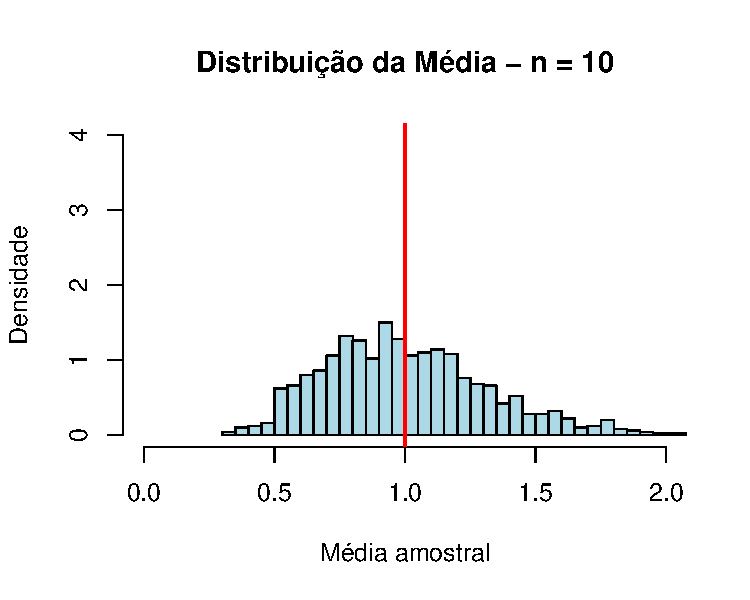
\includegraphics[width=\linewidth]{hist/hist_exp_n10.pdf}
    \end{minipage}
    \begin{minipage}{0.31\textwidth}
        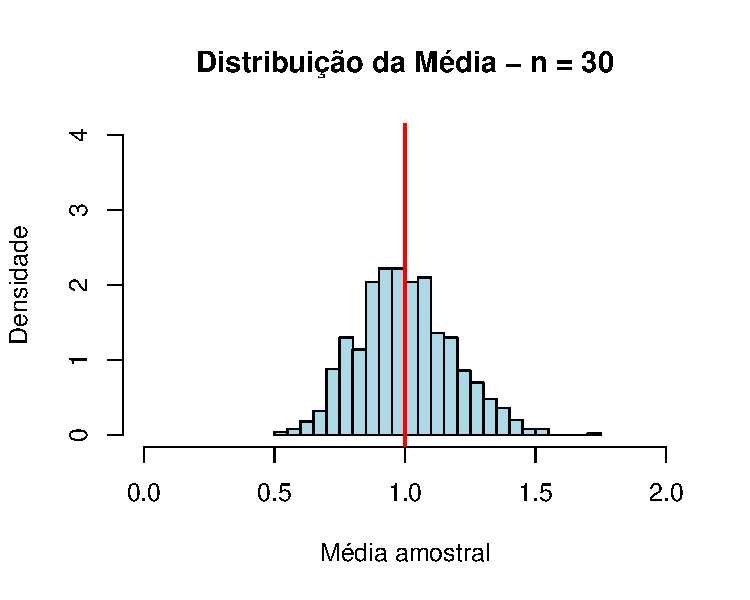
\includegraphics[width=\linewidth]{hist/hist_exp_n30.pdf}
    \end{minipage}\\
    \begin{minipage}{0.31\textwidth}
        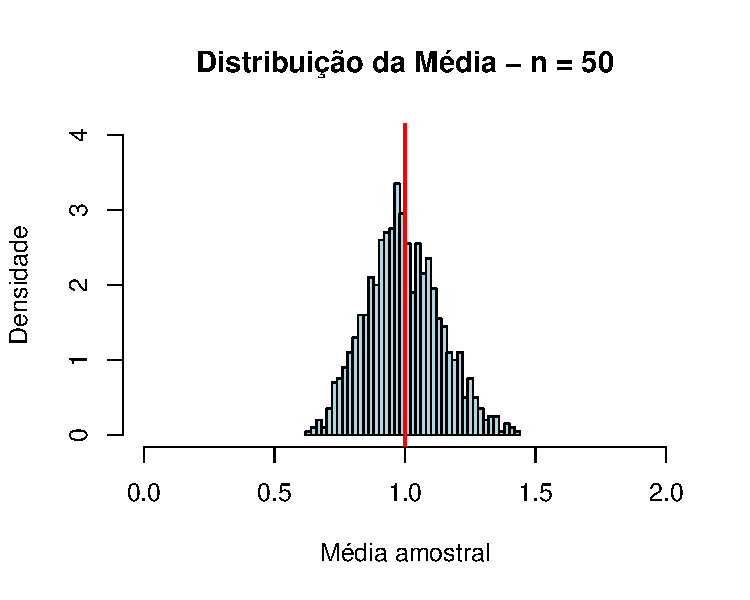
\includegraphics[width=\linewidth]{hist/hist_exp_n50.pdf}
    \end{minipage}
    \begin{minipage}{0.31\textwidth}
        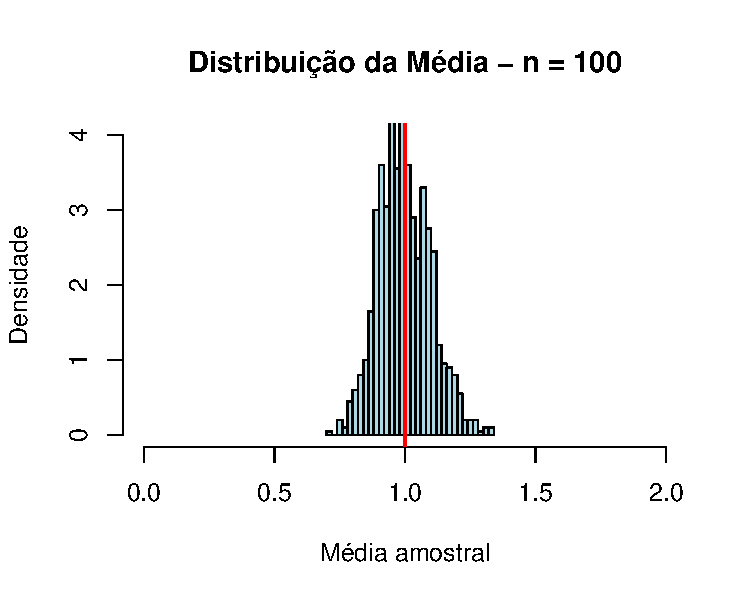
\includegraphics[width=\linewidth]{hist/hist_exp_n100.pdf}
    \end{minipage}
\end{frame}

\begin{frame}{Perguntas}
    \begin{itemize}
        \item \textit{O que acontece com a distribuição das médias amostrais
        quando o tamanho da amostra aumenta?}
        \item \textit{Qual o valor esperado das médias amostrais para cada
        tamanho n considerado?}
        \item \textit{Qual a variância esperada das médias amostrais para cada
        valor de n? A variância diminui com o crescimento de n?}
    \end{itemize}
\end{frame}

\begin{frame}{Conclusão}
    \begin{itemize}
        \item A propaganda da empresa concorrente é enganosa, pois de acordo o
        Teorema Central do Limite (TCL) a probabilidade das entregas serem
        feitas em até um dia é de no máximo 30\%
        \item Assim, como a probabilidade é inferior a 50\% dos pedidos, a
        empresa concorrente não deveria afirmar que grande parte dos seus
        pedidos acontece em menos de um dia
    \end{itemize}
\end{frame}

\end{document}
